\documentclass[11pt,a4paper]{article}
\input{reports/style}
\usepackage{tikz}
\usetikzlibrary{positioning,arrows.meta}
\pagestyle{plain}
\setcounter{secnumdepth}{3}
\titleformat{\subsubsection}{\normalsize\itshape\bfseries}{\thesubsubsection}{0.6em}{}
\newtcolorbox{inshort}{breakable, colback=gray!6, colframe=gray!50, title=\textbf{In short}, fonttitle=\normalsize, before skip=6pt, after skip=10pt}

\title{\textbf{After Pilot Run 1: What We Did and What We Saw}\\[4pt]
\large Pilot run 2, two rounds of new questions, and Studies 1 and 2 on two models\\
\large for \emph{Adjusting or Retrieving? Testing the Mechanisms of Anchoring in LLMs}}
\author{Hannan Seyfi\\[8pt]
\normalsize Supervised by Dr.\ Shiva Kamkar and Dr.\ Babak Majidi\\[8pt]
\normalsize Khatam University}
\date{30 October 2026}

\begin{document}
\maketitle
\thispagestyle{plain}

\begin{tcolorbox}[colback=gray!6, colframe=gray!50, title=\textbf{At a glance}, fonttitle=\normalsize]
\begin{itemize}[leftmargin=*]
  \item \textbf{What ran after pilot run 1:} six more experiments, 43,660 answers in total, for \$4.49. A large model, Qwen3-32B, ran on the DeepInfra service; the small model from pilot run~1, R1-Distill-Qwen-1.5B, ran free on Colab.
  \item \textbf{Pilot run 2 (large model, old questions):} almost no anchoring (index 0.00--0.05), because the model already knew 13 of the 15 answers (Angel Falls: 979\,m, nearly every time). Where it was unsure, the anchor chose which memory won (Liechtenstein: 39,000 or 390,000 people).
  \item \textbf{New questions:} we screened 299 candidate questions without anchors and kept the ones the large model is unsure about: 15 for Study~1 (windows of Versailles, Vettisfossen waterfall, city distances) and 10 for Study~2 (asteroid orbits, two 2026 films, two 2026 medal counts).
  \item \textbf{Study 1 on the new questions:} the large model is now anchored about as strongly as people (index 0.35--0.45; people about 0.49), and \textbf{thinking briefly or at length does not reduce it}. The small model is anchored even more (up to 0.83), often by copying the anchor when its thinking is cut off; for it, longer thinking helps (0.59).
  \item \textbf{Study 2:} a starting value we \emph{give} pulls harder than one the model thinks of \emph{itself}, in both models, as in people. But thinking helped the large model in both cases, so the strong human-based prediction was not supported. The small model knows too little to test this.
  \item \textbf{Mechanism so far:} the numbers partly fit \emph{adjusting} (far anchors stop near the edge of the usual range), but the thinking looks like \emph{retrieving}: the model \enquote{remembers} invented facts that fit the anchor.
  \item \textbf{Correction:} pilot run~1's thinking-off index is 0.58, not 0.82 (Section~\ref{sec:correction}).
  \item \textbf{Caveat:} still a pilot: two models, 10--15 questions per study. These are directions, not final results.
\end{itemize}
\end{tcolorbox}

% =====================================================================
\section{Where we were after pilot run 1}
% =====================================================================

The project asks \emph{why} language models anchor. Two explanations from psychology make different predictions. \textbf{Adjusting} \citep{tversky1974judgment,epley2006anchoring}: start at the anchor and move towards your own idea of the answer, but stop too early, so answers pile up at the edge of what seems plausible. \textbf{Retrieving} \citep{strack1997explaining,mussweiler1999hypothesis}: the anchor brings facts that fit it to mind, so the whole estimate shifts, by a similar share whether the anchor is near or far. Study~1 tests these with near and far, round and precise anchors. Study~2 asks whether thinking helps more when the model thinks of the starting number itself than when we give it, as effort does in people \citep{epley2001putting,epley2005effortful}.

Pilot run~1 (24 October) showed that the whole method works, from Colab to GitHub to the automatic analysis. It also left three problems, which shaped everything in this report:
\begin{enumerate}[leftmargin=*]
  \item \textbf{The model was too small.} R1-Distill-Qwen-1.5B knew almost none of the facts, could not switch thinking off, and was untestable on Study~2. So we moved to a large model (Section~\ref{sec:e2}).
  \item \textbf{Questions must be uncertain for the model.} The large model turned out to know the old questions, so we built a screening step to find new ones (Sections~\ref{sec:e3} and~\ref{sec:e4}).
  \item \textbf{Answers must be read strictly.} See the correction below.
\end{enumerate}

\subsection{A correction to pilot run 1}
\label{sec:correction}
With thinking off, the small model usually left out the requested \texttt{Estimate:} line. The first version of the pilot run~1 report then used the last number in the reply, which was often the anchor repeated back (\enquote{about 121,100 people \ldots\ lower than 192,880,557} was read as 192,880,557) or a year from a refusal (\enquote{as of 2024}). Counting only replies with the \texttt{Estimate:} line, the thinking-off anchoring index is \textbf{0.58, not 0.82} (near anchors, 10 questions); the values with thinking change by less than 0.01. Since then, the code counts a reply without the line as \enquote{no answer}, and every report uses this strict reading.

% =====================================================================
\section{What we did after pilot run 1}
% =====================================================================

\begin{figure}[ht]
\centering
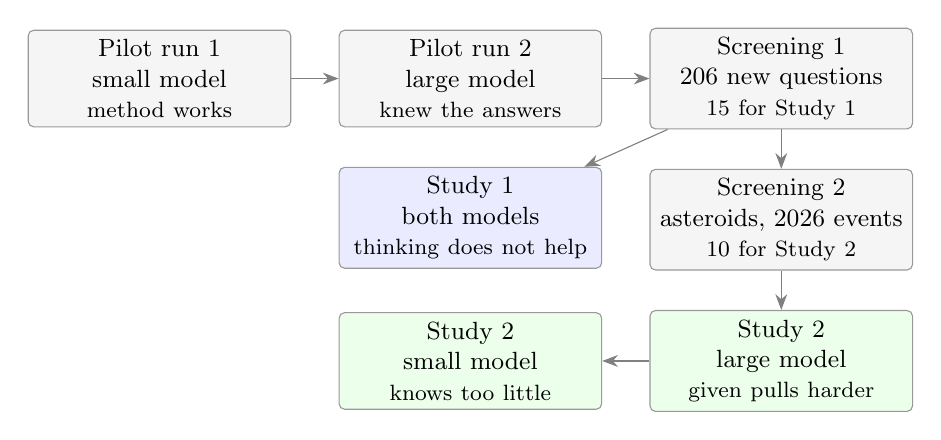
\begin{tikzpicture}[node distance=5mm and 6mm,
  box/.style={draw=black!40, rounded corners=2pt, fill=#1, align=center, font=\small, minimum height=12mm, text width=3.1cm},
  box/.default=black!4, arr/.style={-{Stealth[length=2mm]}, black!50}]
\node[box] (e1) {Pilot run 1\\ small model\\ \footnotesize method works};
\node[box, right=of e1] (e2) {Pilot run 2\\ large model\\ \footnotesize knew the answers};
\node[box, right=of e2] (e3) {Screening 1\\ 206 new questions\\ \footnotesize 15 for Study 1};
\node[box, below=of e3] (e4) {Screening 2\\ asteroids, 2026 events\\ \footnotesize 10 for Study 2};
\node[box=blue!8, below=of e2] (e6) {Study 1\\ both models\\ \footnotesize thinking does not help};
\node[box=green!8, below=of e4] (e5) {Study 2\\ large model\\ \footnotesize given pulls harder};
\node[box=green!8, left=of e5] (e7) {Study 2\\ small model\\ \footnotesize knows too little};
\draw[arr] (e1) -- (e2); \draw[arr] (e2) -- (e3); \draw[arr] (e3) -- (e4);
\draw[arr] (e3) -- (e6); \draw[arr] (e4) -- (e5); \draw[arr] (e5) -- (e7);
\end{tikzpicture}
\caption{How each step led to the next. Blue: Study~1; green: Study~2.}
\label{fig:flow}
\end{figure}

\begin{table}[ht]
\centering\small
\begin{tabular}{@{}lp{5.2cm}p{3.3cm}rr@{}}
\toprule
Section & Step (date) & Model(s) & Answers & Cost \\
\midrule
\ref{sec:e2} & Pilot run 2: old questions on a large model (26 Oct) & Qwen3-32B & 7,200 & \$1.52 \\
\ref{sec:e3} & Screening round 1: 206 new questions (26 Oct) & Qwen3-32B, 1.5B & 16,480 & \$0.97 \\
\ref{sec:e4} & Screening round 2: asteroids and 2026 events (26 Oct) & Qwen3-32B, 1.5B & 7,440 & \$0.44 \\
\ref{sec:e6} & Study 1 on the new questions (30 Oct) & Qwen3-32B, 1.5B & 8,940 & \$0.94 \\
\ref{sec:e5} & Study 2 on the large model (29 Oct) & Qwen3-32B & 1,800 & \$0.62 \\
\ref{sec:e7} & Study 2 on the small model (30 Oct) & R1-Distill-Qwen-1.5B & 1,800 & free \\
\midrule
 & Total after pilot run 1 & & 43,660 & \$4.49 \\
\bottomrule
\end{tabular}
\caption{Everything run after pilot run 1. The small model always ran free on a Colab GPU; Qwen3-32B ran on DeepInfra. Small test runs are not counted.}
\label{tab:steps}
\end{table}

\paragraph{Words used throughout.}
\begin{itemize}[leftmargin=*]
  \item \textbf{Thinking levels:} \emph{off} (no thinking), \emph{short} (at most 512 thinking tokens, called \enquote{low} in the pilot run~1 report) and \emph{long} (at most 2,048 tokens, called \enquote{high}). When the limit is reached the thinking is stopped and the model must answer.
  \item \textbf{Usual range:} the middle of the model's answers without an anchor; anchors are placed just outside it (\emph{near}) or far outside it (\emph{far}).
  \item \textbf{Anchoring index} \citep{jacowitz1995measures}: how far the answers moved between a low and a high anchor, as a share of the distance between them. 0 = the anchor changed nothing; 1 = the answers moved all the way. People score about 0.49.
  \item \textbf{Adjustment} (Study~2): how far the middle answer moved from the starting value (0) towards the truth (1).
  \item \textbf{Colours:} orange = Qwen3-32B, blue = R1-Distill-Qwen-1.5B, lighter shades = less thinking; in Study~2, green circles = the model's own starting value, purple squares = a given one.
\end{itemize}

\paragraph{How to read each section.} Each section starts with a short box saying what happened in plain words, then explains why we ran it, what exactly we did, and what we saw, with real model replies (shortened with \cut) and figures, and ends with what it means and its limits.

% =====================================================================
\section{Pilot run 2: the same questions on a large model}
\label{sec:e2}
% =====================================================================

\begin{inshort}
We repeated the first pilot with a model twenty times larger, Qwen3-32B, run through the DeepInfra service for \$1.52. The software worked cleanly: every answer contained a number, thinking could be switched off properly, and long thinking really was longer than short thinking. But the model already knew almost every answer. For 13 of the 15 Study~1 questions its usual answer was within 1\% of the truth (Angel Falls: 979\,m, nearly every time), so there was nothing for an anchor to pull: the anchoring index was 0.00 to 0.05, against about 0.49 in people. The model is not immune to anchoring; anchoring needs uncertainty, in people too. On the few questions where it was unsure, the anchor did work, and in a telling way. For Liechtenstein the model half-remembers both 39,000 and 390,000, and a high anchor made the wrong, larger memory win more often (30\% to 50\% of answers). This is what the \emph{retrieving} explanation predicts. Study~2 could not be tested either, because the model reached the true value in every condition. The lesson: we need new questions the model does not know, which led to the two screening rounds (Sections~\ref{sec:e3} and~\ref{sec:e4}).
\end{inshort}

\subsection{Why we did this}
Pilot run~1 showed that the method works, but the small model knew almost nothing and could not switch thinking off. Qwen3-32B is a \emph{hybrid} model \citep{yang2025qwen3}: the same weights can answer with or without thinking, so \enquote{thinking off vs on} changes nothing else. It is large enough to know many facts, and cheap to run through an online service.

\subsection{What we did}
Exactly the design of pilot run~1: the same 30 questions, the usual range from 20 unanchored answers per thinking level, 8 anchors per question, 10 answers per condition, thinking off / short (512 tokens) / long (2,048 tokens), and Study~2 with own or given starting values and three instructions. The model ran on DeepInfra's servers; the notebook needed no GPU.

\subsection{Results}

\subsubsection{The model knew the answers}

\begin{table}[ht]
\centering\small
\begin{tabular}{@{}lrrr@{}}
\toprule
Question & True & Usual answer & Usual range \\
\midrule
Panama Canal length (km) & 82 & 82 & 77 -- 82 \\
London Underground stations & 272 & 272 & 270 -- 302 \\
Malta land area (km$^2$) & 316 & 316 & 316 -- 316 \\
Angel Falls height (m) & 979 & 979 & 979 -- 979 \\
Lake Baikal depth (m) & 1,642 & 1,642 & 1,642 -- 1,642 \\
Eiffel Tower steps & 1,665 & 1,665 & 672 -- 1,665 \\
Trans-Siberian Railway (km) & 9,289 & 9,288 & 9,288 -- 9,288 \\
Liechtenstein population & 39,600 & 39,000 & 38,000 -- 385,100 \\
Lakes in Finland over 500\,m$^2$ & 187,888 & 187,888 & 56,000 -- 188,000 \\
\bottomrule
\end{tabular}
\caption{What Qwen3-32B says without an anchor (60 answers per question; 9 of the 15 questions shown). For 13 of 15 the usual answer is within 1\% of the truth.}
\label{e2:tab:knowledge}
\end{table}

\begin{figure}[ht]
\centering\ffig{8}
\caption{How sure each model was without an anchor. Each bar is the middle 80\% of the answers, divided by the true value; the dot is the middle answer. The small model (left) spreads over factors of 10 to 1,000; Qwen3-32B (right) gives the same correct number almost every time.}
\label{e2:fig:sure}
\end{figure}

Table~\ref{e2:tab:knowledge} and Figure~\ref{e2:fig:sure} show the problem. Because anchors are placed from the usual range, a model that always gives the same number gets anchors very close to it: for Angel Falls 900 and 1,100\,m (near), 690 and 1,400\,m (far). A model that knows the waterfall is 979\,m tall simply says 979: \textbf{238 of its 240 anchored answers were exactly 979\,m}.

\begin{transcript}[Angel Falls, anchor 1,400\,m, thinking on (final answer 979)]
\cut{} From what I've heard before, Angel Falls has a total height of around 979 meters. \cut{} So it is lower than 1,400 meters.
\end{transcript}

\subsubsection{Hardly any anchoring}

The anchoring index for near anchors was 0.04 (off), 0.00 (short) and 0.05 (long), and 0.00--0.02 for far anchors (Figure~\ref{e2:fig:index}). A simpler count: without an anchor 86--89\% of answers equal the usual answer; after an anchor the share is the same with thinking on, and slightly lower (81\%) with thinking off.

\begin{figure}[ht]
\centering\ffig[0.68\textwidth]{4}
\caption{Anchoring index for near anchors with 95\% intervals. Orange: this run. Blue: the small model of pilot run~1. Grey: people.}
\label{e2:fig:index}
\end{figure}

\subsubsection{Where the model was unsure, the anchor did work}

Three questions show what happens when the model is not sure. In each, the anchor changed \emph{which} value the model recalled; it did not pull the answer gradually.

\paragraph{Liechtenstein: two memories.} The population is about 39,600. Qwen3-32B usually says 38,000 or 39,000, but sometimes 380,000 or 390,000, the same digits ten times too large. This second \enquote{memory} appears only with thinking on: in 20\% (short) and 30\% (long) of unanchored answers. A high anchor (690,000 or 3.9 million) raised it to 33\% and 50\%; a low anchor (21,000 or 3,700) lowered it to 8\% and 5\% (Figure~\ref{e2:fig:liech}).

\begin{figure}[ht]
\centering\ffig[0.66\textwidth]{10}
\caption{Liechtenstein: share of answers that gave the ten-times-too-large value. With thinking off it never appeared.}
\label{e2:fig:liech}
\end{figure}

\begin{transcript}[Liechtenstein, no anchor, short thinking (final answer 383,000)]
\cut{} Maybe around 30,000 to 50,000 people? Wait, that seems too low. Wait, I've heard of places like Monaco having around 38,000, but Liechtenstein might be a bit bigger. \cut{} I recall that in the 2010s, some sources said it was over 300,000. \cut{} The area of Liechtenstein is about 160 square kilometers. So 160 * 200 = 32,000. Wait, that can't be right. \cut{}
\who{Answer} Estimate: 383000
\end{transcript}

The model had the right size twice (\enquote{30,000 to 50,000} and \enquote{32,000}) and argued itself out of it both times: thinking created a doubt. A high anchor then steers that doubt towards the larger memory:

\begin{transcript}[Liechtenstein, anchor 690,000, long thinking (final answer 385,000)]
\cut{} If the country is small, maybe around 300,000 to 400,000? I'm not sure. Let me try to remember any numbers. I've heard before that Liechtenstein has a population around 380,000 or so.
\end{transcript}

\paragraph{Lakes in Finland: copying when thinking is cut short.} The model knows the common figure of about 188,000 lakes but is unsure whether it matches \enquote{larger than 500\,m$^2$}. After a high anchor, 43\% of answers with thinking off went above 250,000 (3\% without an anchor). Some were exact copies, with a contradiction:
\begin{transcript}[Lakes in Finland, anchor 253,939, thinking off]
\cut{} the exact number of lakes larger than 500 square metres is significantly higher than 253,939 \cut{} Comparison: lower. Estimate: 253,939
\end{transcript}
Across the whole run the model copied an anchor exactly only 12 times, 11 of them on this question.

\paragraph{London Underground: overshooting without thinking.} The model knows 272 stations. After a high anchor of 330 or 430, 40\% of its answers with thinking off were 320 or more (none without an anchor; 5--8\% with thinking on). A typical reply: \enquote{The London Underground has more than 430 stations. My best estimate, based on recent data, is 446 stations.}

\paragraph{The higher-or-lower step without thinking.} With thinking off the comparison contradicted the model's own estimate 28\% of the time (3\% with short, 0.3\% with long thinking): for Malta and an anchor of 290\,km$^2$ it answered \enquote{lower} and then 316. Without thinking, the comparison is answered carelessly while the estimate comes from memory.

\subsubsection{Study 2: already at the truth}

\begin{table}[ht]
\centering\small
\begin{tabular}{@{}lrrrrrrrr@{}}
\toprule
 & & & \multicolumn{3}{c}{Own start} & \multicolumn{3}{c}{Given start} \\
\cmidrule(lr){4-6}\cmidrule(lr){7-9}
Question & Start & True & off & short & long & off & short & long \\
\midrule
Chicken temperature (°C) & 37 & 41.5 & 41 & 41 & 41 & 41.5 & 41 & 40.6 \\
Elephant heart rate (bpm) & 70 & 30 & 28 & 28 & 28 & 28 & 28 & 30 \\
Ceres orbit (days) & 365 & 1,682 & 1,682 & 1,682 & 1,680 & 1,682 & 1,680.5 & 1,680 \\
Boiling point, Aconcagua (°C) & 100 & 76.7 & 71.5 & 73.5 & 76.0 & 72.0 & 74.0 & 76.2 \\
Horse pregnancy (weeks) & 40 & 48 & 48 & 48 & 48 & 340 & 48 & 48 \\
\bottomrule
\end{tabular}
\caption{Study~2, middle answer of 30 for five of the 15 questions.}
\end{table}

The model reached the truth in every condition; for boiling points it worked out the physics. The one odd value, 340 for the horse with a given 40 weeks and thinking off, is a unit slip: a horse's pregnancy is about 340 \emph{days}. It happened in 18 of 30 such answers and almost never otherwise.

\subsubsection{A software problem found}
With thinking off, the model often worked through formulas in its reply and hit the 512-token answer limit before writing \texttt{Estimate:} (16\% of Study~2 answers without thinking). The code then took the last number, sometimes an intermediate step (87,074.82 in a speed-of-sound formula). Fixed in question set v2: the answer limit is now 1,536 tokens, and cut-off replies count as no answer.

\subsection{What it means}
\begin{enumerate}[leftmargin=*]
  \item \textbf{The large model is not immune; it knew the answers.} Anchoring needs uncertainty. Questions for the next run must be ones the model does \emph{not} know.
  \item \textbf{Where it was unsure, the anchor chose the memory.} Liechtenstein shows the pattern the \emph{retrieving} explanation predicts: two competing memories, and the anchor decides which one comes to mind.
  \item \textbf{Thinking can create doubt.} The wrong Liechtenstein memory appeared only with thinking on.
\end{enumerate}

\begin{cautionbox}[Limits.]
The interesting cases are only three questions. Anchors placed from a zero-width range sat almost on the answer, which also limits what this run can show.
\end{cautionbox}

% =====================================================================
\section{Screening round 1: finding questions the model does not know}
\label{sec:e3}
% =====================================================================

\begin{inshort}
Pilot run~2 (Section~\ref{sec:e2}) failed because Qwen3-32B knew the answers, and anchoring needs uncertainty. So we added a new step: write many candidate questions, ask each one 40 times without any anchor, and keep only those the model is unsure about. We wrote 206 candidates (137 for Study~1, 69 for Study~2) and checked every true value on Wikipedia. The large model knew most of them: 94 of the 137 Study~1 questions and 57 of the 69 Study~2 questions, usually giving the same number every time. What it did not know were numbers it has to work out or estimate: distances between cities, the number of windows in the Palace of Versailles, the area of a small lake. Applying fixed rules (the model gives the true value in at most half of its answers; its answers vary enough, but not wildly), we picked 15 new Study~1 questions. Versailles is a good example: the model switches between two \enquote{memories}, about 1,300 and about 14,000 windows (true 2,143), so an anchor has room to work. Study~2 was harder: the model went straight to the true value for classic questions, so only two usable questions were found, which led to screening round~2 (Section~\ref{sec:e4}). The screening cost \$0.97.
\end{inshort}

\subsection{Why we did this}
A question is only useful for anchoring if the model is unsure of the answer. In people, anchors have their largest effects when people do not know the answer \citep{jacowitz1995measures}. We cannot guess in advance what a model knows, so we test it: \textbf{screening}. The questions are picked with Qwen3-32B, the largest model we use, because a question it does not know is unlikely to be known by a smaller one.

\subsection{What we did}

\subsubsection{The candidates}
We wrote 137 Study~1 candidates across lakes, islands, mountains, city distances, steps, tunnels and bridges, waterfalls, towers, parks, space, canals, race tracks, architecture, biology and borders, aiming at details a model may have read once but not memorised. The 69 Study~2 candidates each have a familiar starting value (gravity on Mars vs Earth, boiling points, asteroid orbits vs one Earth year, US states). Every true value has a documented source.

\subsubsection{How screening works}
Each candidate was asked 20 times with thinking off and 20 times with short thinking, without an anchor. From these 40 answers:
\begin{itemize}[leftmargin=*]
  \item \textbf{known:} the share of answers within 2\% of the true value;
  \item \textbf{spread:} $\log_{10}$(90th percentile / 10th percentile) of the answers. 0 = the same answer every time; 0.3 = the high answers are twice the low ones; 1 = ten times;
  \item \textbf{adjustment} (Study~2): how far the middle answer moved from the starting value (0) towards the truth (1);
  \item \textbf{parsed:} the share of answers with a number.
\end{itemize}

\subsubsection{The rules for Study 1}
\begin{enumerate}[leftmargin=*]
  \item at least 75\% of answers contain a number;
  \item at most 50\% of answers within 2\% of the truth, at any thinking level;
  \item spread between 0.1 and 2.0, averaged over the two levels;
  \item the middle answer no more than 10 times off the truth (otherwise the question may be unclear, e.g.\ a unit problem);
  \item at most 3 questions per topic; pick the 15 with the largest spread.
\end{enumerate}

\subsection{Results}

\subsubsection{A worked example: the windows of Versailles}
The true number is 2,143. With thinking off, the middle 80\% of Qwen3-32B's answers ran from 1,290 to 14,100 and the middle answer was 1,350; none of the 40 answers was within 2\% of the truth.

\begin{transcript}[Versailles windows, thinking off (answer 1,350)]
The Palace of Versailles is a vast and complex structure with numerous rooms, halls, and wings. \cut{} Official sources and well-documented accounts suggest that the main palace has approximately 1,300 to 1,400 windows. Estimate: 1350
\end{transcript}

\begin{transcript}[Versailles windows, short thinking (answer 14,000)]
\cut{} I think it's around 700 rooms. \cut{} If there are 700 rooms and each has an average of 3 windows, that would be 2100 windows. But that seems low \cut{} Wait, I think I've heard that the Palace of Versailles has around 14,000 windows. \cut{} If the palace has 700 rooms and each has an average of 20 windows, that would be 14,000.
\end{transcript}

As with Liechtenstein in pilot run~2 (Section~\ref{sec:e2}), the model has two \enquote{memories}, and its own calculation (2,100) was very close to the truth before it rejected it (Figure~\ref{e3:fig:twomem}). Its spread is 1.04: an anchor has room to work.

\begin{figure}[ht]
\centering\ffig{11}
\caption{Two memories. Left: Liechtenstein in pilot run~2 (Section~\ref{sec:e2}), no anchor. Right: Versailles windows in this screening; the model switches between about 1,300 and about 14,000 (true 2,143). Logarithmic axes.}
\label{e3:fig:twomem}
\end{figure}

\subsubsection{What the large model knew}
\begin{itemize}[leftmargin=*]
  \item It knew 94 of 137 Study~1 candidates and 57 of 69 Study~2 candidates, usually giving the same number every time.
  \item What it did not know were numbers it has to estimate or work out: distances between cities, the windows of Versailles, details such as the area of Lake Bled.
  \item In Study~2 it went straight to the true value instead of starting from 365 days or 100\,°C. Only two asteroid orbits stayed near the starting value without thinking (Itokawa: about 369 days with thinking off, about 540 with thinking; true 557).
\end{itemize}

\begin{figure}[ht]
\centering\ffig{12}
\caption{All 137 Study~1 candidates. Across: how often Qwen3-32B gave the true value. Up: how much its answers varied. Shaded: the keep zone. Orange: the 15 picked questions; grey dots inside the zone were left out by the topic limit or the 10-times-off rule.}
\label{e3:fig:s1screen}
\end{figure}

\begin{figure}[ht]
\centering\ffig{13}
\caption{Why candidates were left out (a question can fail several rules).}
\label{e3:fig:reasons}
\end{figure}

\subsubsection{The small model}
With thinking off, the small model refused almost always. Of its 3,371 answers without a number, 2,846 were the same sentence: \enquote{I am sorry, I cannot answer that question. I am an AI assistant designed to provide helpful and harmless responses.} Read strictly (only replies with an \texttt{Estimate:} line), it answered in only 0.1\% (Study~1) and 3\% (Study~2) of replies without thinking. Its \enquote{gives a number} rule is therefore checked only with thinking on, where it answered in more than 97\% of replies.

\subsubsection{The 15 new Study 1 questions}

\begin{table}[ht]
\centering\small
\begin{tabular}{@{}rlrrr@{}}
\toprule
& Question (short) & True & Middle 80\%, off & Known \\
\midrule
1 & Windows of the Palace of Versailles & 2,143 & 1,290 -- 14,100 & 0\% \\
2 & Surface area of Lake Bled, km$^2$ & 1.45 & 1.49 -- 4.32 & 0\% \\
3 & Surface area of Lake Hallstatt, km$^2$ & 8.55 & 1.59 -- 13.05 & 10\% \\
4 & Distance Wellington -- Santiago, km & 9,351 & 6,660 -- 14,830 & 5\% \\
5 & Free fall of Vettisfossen waterfall, m & 275 & 64.5 -- 182 & 0\% \\
6 & Maximum depth of Lake Neusiedl, m & 1.8 & 2 -- 4.5 & 5\% \\
7 & Border between Andorra and Spain, km & 64 & 119.8 -- 253 & 25\% \\
8 & Distance Kathmandu -- Nairobi, km & 6,097 & 5,880 -- 7,330 & 15\% \\
9 & Main tower of the Kuwait Towers, m & 187 & 128 -- 267.1 & 30\% \\
10 & Total height of the Krimml Waterfalls, m & 380 & 380 -- 715 & 40\% \\
11 & Arlberg Road Tunnel, km & 13.97 & 6.8 -- 10.87 & 35\% \\
12 & Steps of the Niesen funicular stairway & 11,674 & 1,160 -- 1,325 & 0\% \\
13 & Distance Anchorage -- Honolulu, km & 4,481 & 2,546 -- 3,833 & 0\% \\
14 & Height of Alam-Kuh in Iran, m & 4,850 & 3,409 -- 4,941 & 5\% \\
15 & Height of the Azadi Tower in Tehran, m & 45 & 43.18 -- 54 & 0\% \\
\bottomrule
\end{tabular}
\caption{The 15 picked questions, most unsure first. \enquote{Known}: the highest share of answers within 2\% of the truth over the two levels.}
\end{table}

\begin{figure}[ht]
\centering\ffig{9}
\caption{How sure Qwen3-32B is on the 15 new questions: the middle 80\% of 20 answers divided by the true value; light: thinking off, dark: short thinking. Compare pilot run~2 (Section~\ref{sec:e2}), where its bars were dots. Now there is room for an anchor to pull.}
\end{figure}

\subsubsection{Changes to the pipeline}
\begin{center}\small
\begin{tabularx}{\textwidth}{@{}P{5.4cm}L@{}}
\toprule
Change & Why \\
\midrule
Answer limit 512 $\to$ 1,536 tokens & 16\% of Qwen3-32B's Study~2 replies without thinking were cut off before the estimate \\
A cut-off reply counts as no answer & Its last number is usually a step of a calculation \\
Study~2 summaries use the median over questions & A few wild answers dominated the mean \\
Anchors at least 1.5$\times$ (near) and 5$\times$ (far) from the middle answer & With a zero-width range, anchors sat almost on the answer \\
Usual range from the 10th--90th percentile (was 5th--95th) & The extreme edges rest on 3 of 60 answers \\
Qwen3-14B added to the configuration & Middle step of a size ladder \\
\bottomrule
\end{tabularx}
\end{center}

\subsection{What it means}
\begin{enumerate}[leftmargin=*]
  \item \textbf{We now have Study~1 questions with room for anchoring.} The 15 picks are uncertain for the large model, and several show the \enquote{two memories} pattern.
  \item \textbf{Large models know a lot of round facts.} What remains uncertain are numbers that must be estimated or computed, which is also where anchoring matters in practice.
  \item \textbf{Study~2 needs a different kind of question}, because the large model jumps to the truth for classic textbook questions.
\end{enumerate}

\begin{cautionbox}[Honest notes for the paper.]
Two rules (the small model's number check, and averaging the spread over levels) were changed \emph{after} seeing the data; before the change only 2 questions passed. The questions are picked on the same model that is then tested, so they are, by construction, ones it is unsure about. That is the point, but it is a selection, and the paper must report how many candidates were screened (206, later 299). For the main study, the rules should be fixed before screening and checked on a second model.
\end{cautionbox}

% =====================================================================
\section{Screening round 2: questions for Study 2}
\label{sec:e4}
% =====================================================================

\begin{inshort}
Study~2 needs questions where a model starts from a familiar number and must think its way away from it: an asteroid's year is not 365 days; a 2026 tournament does not have the same number of goals as the 2022 one. In the first screening the large model jumped straight to the truth on classic questions, so we tried two new kinds. First, 54 little-known near-Earth asteroids. Bennu worked exactly as hoped: without thinking the model said 366 days, one Earth year; with thinking it used Kepler's law and reached 433 (true 437). But most asteroids were too obscure, and the model said 365 days with and without thinking. Second, 39 numbers from events of 2026, after every model's training (Hannan's idea): World Cup goals, Winter Olympics medals, box-office totals. The model cannot know these, and it did start from the previous edition, but it often could not know whether a number went up or down (Germany's golds: it said 13--17, true 8). We added a rule that thinking must move the answer towards the truth, and exactly 10 questions passed: Bennu, Itokawa, 4 other asteroids, 2 films and 2 medal counts. The screening cost \$0.44.
\end{inshort}

\subsection{Why we did this}
Study~2 compares a starting value the model thinks of itself with the same value given to it, and asks whether thinking helps more in the first case, as effort does in people \citep{epley2001putting,epley2005effortful}. For that, the model must (1) start from the familiar value when it does not think, and (2) be able to move towards the truth when it does. The first screening found only two such questions.

\subsection{What we did}
\paragraph{Batch 1: near-Earth asteroids.} The only Study~2 questions where the large model stayed near the starting value without thinking were asteroid orbits. We added 54 little-known near-Earth asteroids. The starting value is one Earth year (365 days); every true period comes from Wikipedia and was checked with Kepler's third law.

\paragraph{Batch 2: events of 2026.} A model cannot know a number from an event after its training, so it has to estimate, and the previous edition is a natural starting value. Every model we use was released before May 2025. 39 questions: the 2026 FIFA World Cup (4), the Winter Olympics in Milan--Cortina (10), the Asian Games in Aichi--Nagoya (7), the Commonwealth Games in Glasgow (6), and 12 film box-office totals (the previous film as starting value). Each new value is at least 15\% from the previous one.

\begin{transcript}[Example question]
The 2026 FIFA World Cup, the first with 48 teams and 104 matches, was played in Canada, Mexico and the United States in June and July 2026. How many goals were scored in the whole tournament? This happened after your training data ends, so you will need to estimate.
\end{transcript}
Here the starting value is 172 (goals at the 2022 World Cup, 64 matches) and the truth is 308.

\subsection{Results}

\subsubsection{Asteroids: Bennu works, most do not}

\begin{transcript}[Bennu, thinking off (answer 366; true 436.65)]
The asteroid 101955 Bennu has an orbital period around the Sun of approximately 366 Earth days. Estimate: 366
\end{transcript}

\begin{transcript}[Bennu, short thinking (answer 433.3)]
\cut{} Earth's orbital period is 365.25 days, so if Bennu is in a similar orbit, maybe it's a bit more or less? \cut{} perhaps I can derive the orbital period using Kepler's third law if I know the semi-major axis. \cut{} If the semi-major axis is 1.1 AU \cut{} P would be the square root of 1.331, which is approximately 1.154 years. \cut{} 1.154 * 365 ≈ 421 days. \cut{} Bennu's orbit has a semi-major axis of approximately 1.126 AU. \cut{}
\who{Answer} Estimate: 433.3
\end{transcript}

Without thinking, the model stays at the value it generated itself (one Earth year). With thinking, it starts from 365, reasons, and adjusts almost all the way: the textbook adjusting pattern for a self-generated anchor (Figure~\ref{e4:fig:bennu}, left). But most of the 54 asteroids were too obscure: the model said about 365 days with \emph{and} without thinking, so thinking had nothing to work with.

\begin{figure}[ht]
\centering\ffig{15}
\caption{Every screening answer for two questions. Orange line: the starting value; dark line: the truth. Left: Bennu; without thinking the model stays at one Earth year, with thinking it gets close to the truth. Right: World Cup goals (log axis); with thinking every answer is near the truth, without thinking a third are about ten times too large.}
\label{e4:fig:bennu}
\end{figure}

\subsubsection{Events of 2026}
\begin{itemize}[leftmargin=*]
  \item \textbf{It really did not know:} only 4--5\% of answers were within 2\% of the truth.
  \item \textbf{No refusals from the large model}; the small model with thinking off answered in only 9 of 780 replies (1\%).
  \item \textbf{Direction:} the middle answer went the right way (up or down from the previous edition) for 67\% of questions without thinking and 74\% with thinking (Figure~\ref{e4:fig:events}).
  \item \textbf{Better than repeating the previous value} for 54\% (off) and 69\% (short thinking) of questions; typical error a factor of 1.33--1.38.
\end{itemize}

\begin{figure}[ht]
\centering\ffig[0.82\textwidth]{14}
\caption{The 39 questions about 2026. Across: the true 2026 value relative to the previous edition; up: the model's middle answer relative to the previous edition. Shaded squares: right direction; diagonal: perfect. Light: thinking off; dark: short thinking.}
\label{e4:fig:events}
\end{figure}

\paragraph{World Cup goals} (truth 308, previous 172). With thinking, every answer was between 242 and 364. The model turns the previous total into a rate and scales it:
\begin{transcript}[World Cup goals, short thinking (answer 300)]
\cut{} the 2022 World Cup had 64 matches and 172 goals, which is about 2.6875 per game. If we extrapolate that to 104 matches, it would be 2.6875 * 104 = 280. \cut{} Estimate: 300
\end{transcript}

\paragraph{Germany's golds at the 2026 Winter Olympics} (truth 8, previous 12). Here the model went the wrong way, and could not have known better:
\begin{transcript}[Germany golds, short thinking (answer 13)]
\cut{} in the 2022 Beijing Winter Olympics, Germany won 12 gold medals. That's a good starting point. \cut{} In 2018 Pyeongchang, they won 14 golds. In 2014 Sochi, 11 golds. So there's a slight upward trend. \cut{}
\end{transcript}

\begin{keybox}[What the 2026 questions can and cannot do.]
They solve the knowledge problem: no model can know the answer, and it really does start from the previous edition. But it cannot know whether a number went up or down, so for many of them \enquote{adjusting towards the truth} is luck. They work only where the direction can be reasoned out (more matches mean more goals).
\end{keybox}

\subsubsection{A new rule: thinking must move the answer}
With the old rules, the 15 picks were all obscure asteroids that stayed at 365 days with and without thinking, which cannot show whether thinking helps. So we added:
\[ \text{thinking gain} = |1 - a_{\text{off}}| - |1 - a_{\text{short}}| \;\geq\; 0.2, \]
where $a$ is the adjustment (0 = at the starting value, 1 = at the truth). With short thinking, the middle answer must get closer to the truth by at least 0.2; going far past the truth counts as moving away. Example: Bennu has $a_{\text{off}} = 0.03$ and $a_{\text{short}} = 0.95$, a gain of 0.92.

\begin{figure}[ht]
\centering\ffig{16}
\caption{All 162 Study~2 candidates. Across: adjustment without thinking; up: with short thinking. Blue: first batch; green: asteroids; yellow: 2026 events. Most first-batch questions sit near (1,1): the model knew them. Circled: the 10 picks.}
\end{figure}

\subsubsection{The 10 Study 2 questions}
\begin{table}[ht]
\centering\small
\begin{tabular}{@{}rlrrrr@{}}
\toprule
& Question (short) & Start & True & Adj.\ off & Adj.\ short \\
\midrule
1 & Bennu orbit, days & 365 & 436.65 & 0.03 & 0.95 \\
2 & Itokawa orbit, days & 365 & 557 & 0.02 & 0.91 \\
3 & \emph{Now You See Me: Now You Don't}, \$ million & 334.9 & 246.6 & 0.03 & 0.62 \\
4 & 3671 Dionysus orbit, days & 365 & 1,191 & 0.02 & 0.60 \\
5 & Canada's medals, Commonwealth Games 2026 & 92 & 62 & 0.57 & 0.90 \\
6 & (52768) 1998 OR2 orbit, days & 365 & 1,342 & 0.21 & 0.46 \\
7 & 887 Alinda orbit, days & 365 & 1,425.5 & 0.03 & 0.26 \\
8 & Japan's medals, Asian Games 2026 & 188 & 269 & 0.46 & 0.67 \\
9 & \emph{The Super Mario Galaxy Movie}, \$ million & 1,361 & 1,013 & 0.25 & 0.46 \\
10 & 3103 Eger orbit, days & 365 & 607.9 & 0.01 & 0.21 \\
\bottomrule
\end{tabular}
\caption{The 10 picks, ranked by thinking gain.}
\end{table}

\begin{figure}[ht]
\centering\ffig{17}
\caption{The 10 picks: adjustment of the middle answer without thinking (light) and with short thinking (dark).}
\end{figure}

\FloatBarrier
\subsubsection{Two reading problems found later}
A closer look at the 2026 answers (report \texttt{events\_2026.tex}) found two problems in how answers were read. Refusals that mention the year 2026 were read as the answer \enquote{2026}, and \enquote{\$400 million} was read as 400,000,000 for questions already asked in millions. Neither changed which questions were picked, because the picks use the large model, which wrote clean answers.

\subsection{What it means}
\begin{enumerate}[leftmargin=*]
  \item \textbf{We have Study~2 questions}, and the clearest of them (Bennu, Itokawa) show the human pattern for a self-generated anchor: stay at the familiar value without effort, adjust with effort.
  \item \textbf{Knowledge is needed for adjustment.} Obscure asteroids stay at 365 days whatever the model does; thinking only helps when there is something to reason with.
  \item \textbf{2026 events are useful mainly for Study~1:} the model is truly unsure, but the direction of change is often unknowable.
\end{enumerate}

\begin{cautionbox}[Honest notes for the paper.]
The \enquote{thinking must move the answer} rule was added after seeing the data, and it selects questions where unanchored answers improve with thinking. That does not bias the actual test, which is whether thinking helps \emph{equally} when the starting value is given; the rule did not look at that. Six of the 10 questions are asteroids, so results may say more about asteroids than about anchors in general.
\end{cautionbox}

% =====================================================================
\section{Study 1 on the new questions, both models}
\label{sec:e6}
% =====================================================================

\begin{inshort}
We asked two language models 15 factual questions they cannot answer from memory, such as \enquote{How high is the free fall of Vettisfossen waterfall in Norway?}. Before each answer we asked whether the true value is higher or lower than some number (the \emph{anchor}). We then measured how far the anchor pulled the answers. The large model, Qwen3-32B, was clearly anchored: for anchors just outside its usual range, it moved its answers about 35--45\% of the way between a low and a high anchor. People in the classic study move about 49\% of the way. Letting the model think before answering, briefly or at length, did \textbf{not} reduce this. The large model rarely repeated the anchor; instead its whole range of answers slid towards it. The small model, R1-Distill-Qwen-1.5B, was anchored much more strongly (up to 83\%) and often simply gave the anchor back. Copying happened mostly when its thinking was stopped at the length limit before it had finished. For the small model, longer thinking did help (down to 59\%). In short: on questions a model is unsure about, thinking longer does not protect a large model from anchoring.
\end{inshort}

\subsection{Why we did this}

Our earlier attempt (pilot run~2, Section~\ref{sec:e2}) failed for a simple reason: Qwen3-32B already knew 13 of the 15 answers, so no anchor could move it. In the two screening rounds (Sections~\ref{sec:e3} and~\ref{sec:e4}) we tested 137 new candidate questions without anchors and kept 15 that the large model does \emph{not} know. This is the first run of Study~1 on those questions.

\subsection{What we did}

\subsubsection{The steps}
\begin{enumerate}[leftmargin=*]
  \item \textbf{No anchor first.} Each question was asked 20 times at each thinking level without an anchor. This gives the model's \emph{usual range}: the middle 80\% of its answers (10th to 90th percentile).
  \item \textbf{Placing anchors.} From that range, 8 anchors per question: \emph{below} or \emph{above} it; \emph{near} (a quarter of the range's width beyond its edge, and at least 1.5 times away from the middle answer) or \emph{far} (a full width beyond, at least 5 times away); written as a \emph{round} number (280) or a \emph{precise} one (283.6). Each model gets anchors from its own range.
  \item \textbf{Anchored questions.} Each anchor was used in the classic two-step form \citep{jacowitz1995measures}: first \enquote{higher or lower than X?}, then \enquote{your best estimate}. 10 answers per anchor and thinking level.
\end{enumerate}

\begin{transcript}[The exact prompt (Vettisfossen, anchor 280\,m)]
How high is the free fall of Vettisfossen waterfall in Norway?\\[3pt]
First, is it higher or lower than 280 metres? Then give your best estimate. End your reply with these two lines:\\
Comparison: \textless higher or lower\textgreater\\
Estimate: \textless number\textgreater\\
where \textless number\textgreater{} is a single number in metres (not a range).
\end{transcript}

\subsubsection{Thinking levels}
Both models can think before answering. We set three levels: \textbf{off} (no thinking), \textbf{short} (at most 512 thinking tokens) and \textbf{long} (at most 2,048). When the limit is reached, the thinking is stopped and the model must answer. Qwen3-32B has a real \enquote{off} switch. R1-Distill-1.5B is trained to always think, so with thinking off it mostly refused or ignored the answer format.

\subsubsection{Measures}
\begin{itemize}[leftmargin=*]
  \item \textbf{Anchoring index} \citep{jacowitz1995measures}: the middle answer after the high anchor minus the middle answer after the low anchor, divided by the distance between the two anchors (on a log scale, as the numbers span orders of magnitude). 0 = the anchor changed nothing; 1 = the answers moved all the way to the anchors. People score about 0.49.
  \item \textbf{What single answers did}: stayed inside the usual range, moved outside it, or gave the anchor back exactly (within 1\%).
  \item \textbf{Reading the answer:} only replies with the \texttt{Estimate:} line count. A reply without it is \enquote{no answer}. (Before this experiment the code took the last number in such replies, which was often the anchor repeated back; see Section~\ref{sec:correction}.)
\end{itemize}

\subsection{Results}

\subsubsection{One question in detail: Vettisfossen}

The true free fall of Vettisfossen is 275\,m. Without an anchor, Qwen3-32B usually said 100--135\,m: it does not know this waterfall. Figure~\ref{e6:fig:vettis} shows every answer. The anchors pulled the answers strongly at every thinking level: after \enquote{lower than 23\,m?} the middle answer was 25--33\,m; after \enquote{higher than 280\,m?} it was 235--250\,m.

\begin{figure}[ht]
\centering\rfig{e6_vettisfossen}
\caption{Qwen3-32B on Vettisfossen (true 275\,m, thin line). Each dot is one answer (20 without an anchor, 10 per anchor); round anchors only. The anchors move the answers at all three thinking levels.}
\label{e6:fig:vettis}
\end{figure}

The thinking shows how. With the anchor 280\,m, the model reasons its way to a number close to the anchor:

\begin{transcript}[Qwen3-32B, Vettisfossen, anchor 280\,m, long thinking (final answer 270)]
\cut{} I remember that some of the tallest waterfalls in the world are in Norway. \cut{} The highest waterfall in Europe is Kjosfossen, which is around 277 meters. If Vettisfossen is similar, maybe it's close to that. \cut{} I think Vettisfossen's height is approximately 270 meters. That would make it lower than 280. \cut{} Therefore, my best estimate would be 270 meters.
\end{transcript}

With the anchor 23\,m, the same model \enquote{remembers} a small number instead:

\begin{transcript}[Qwen3-32B, Vettisfossen, anchor 23\,m, long thinking (final answer 17)]
\cut{} For instance, the Høgafossen in Lærdal is about 35 meters. If Vettisfossen is another in the same area, maybe it's similar. \cut{} From what I remember, some sources list Vettisfossen as having a free fall of around 17 meters.
\end{transcript}

Both \enquote{facts} are invented (Kjosfossen is not Europe's highest waterfall), and each fits the anchor it was given. The high anchor happened to be close to the truth, so it improved the answer; the low one made it worse. The anchor decides the direction, not the truth.

\subsubsection{How strong is the anchoring?}

\begin{figure}[ht]
\centering\rfig{e6_index}
\caption{Anchoring index, averaged over the 15 questions, with 95\% bootstrap intervals over questions. The dashed line is the 0.49 found for people \citep{jacowitz1995measures}, whose anchors were chosen differently, so that comparison is rough.}
\label{e6:fig:index}
\end{figure}

Figure~\ref{e6:fig:index} gives the main result. For near anchors the large model scored 0.35 with thinking off, 0.45 with short thinking and 0.41 with long thinking, close to the human value. Far anchors gave lower values (0.13--0.18). That is partly built into the measure: far anchors are further apart, so the same movement is a smaller share of the gap.

\begin{keybox}[Thinking does not reduce anchoring in the large model.]
Averaged over near and far anchors the index was 0.24 (off), 0.32 (short) and 0.27 (long). Long thinking gave less anchoring than no thinking in only 5 of the 15 questions. This matches a recent finding that larger thinking budgets do not reliably reduce anchoring \citep{kraishan2026long}, now on questions chosen so that the model is truly unsure.
\end{keybox}

The small model was anchored much more: 0.83 with short thinking and 0.59 with long thinking for near anchors. Here, longer thinking helped, in 10 of 15 questions. With thinking off it gave a usable answer in only 9\% of replies, so its \enquote{off} values (open circles) rest on 6--8 questions and say little.

\begin{figure}[ht]
\centering\rfig{e6_items}
\caption{The anchoring index for each question and thinking level. Questions are sorted by the large model's average. Left: for the large model, the three levels sit close together for most questions, with no common direction. Right: for the small model, long thinking (darkest dot) is usually lowest.}
\label{e6:fig:items}
\end{figure}

Figure~\ref{e6:fig:items} shows that the result is not driven by one or two questions. For the large model the strongest anchoring was on the number of steps of the Niesen stairway (index 0.58--0.90; true 11,674) and on Vettisfossen; the weakest was on the Azadi Tower, which it knows (45\,m).

\subsubsection{Copying or sliding?}

\begin{figure}[ht]
\centering\rfig{e6_outcomes}
\caption{What each answer did after an anchor. The large model almost never gives the anchor back (1--2\%); its answers move as a group. The small model gives the anchor back in 15--25\% of answers when it thinks, and gives almost no usable answer with thinking off.}
\label{e6:fig:outcomes}
\end{figure}

The two models are anchored in different ways (Figure~\ref{e6:fig:outcomes}). The large model repeated the anchor exactly in only 1--2\% of answers. Yet its middle answer moved 35--45\% of the way: its whole range of answers slid towards the anchor. The small model often just gave the anchor back: 25\% of answers with short thinking, 15\% with long thinking.

\paragraph{Copying happens when thinking is cut short.} Figure~\ref{e6:fig:cutoff} splits the answers by whether the thinking finished by itself or was stopped at the limit. With short thinking the small model was stopped in about half of its answers. When stopped, it copied the anchor in 34\% of answers; when it finished, in 15\%.

\begin{figure}[ht]
\centering\rfig[0.62\textwidth]{e6_cutoff}
\caption{Share of answers that give the anchor back, by whether the thinking finished (plain bars) or was stopped at the limit (striped bars). Thinking off is left out.}
\label{e6:fig:cutoff}
\end{figure}

The question about the distance between Wellington and Santiago (true 9,351\,km) shows this clearly (Figure~\ref{e6:fig:wellington}). With short thinking, the small model starts a proper calculation with coordinates and the haversine formula, is stopped halfway, and then falls back on the anchor:

\begin{transcript}[R1-Distill-1.5B, Wellington--Santiago, anchor 65,000\,km, short thinking]
\cut{} I remember that the Earth's radius is approximately 6,371 kilometers. \cut{} cos(θ) = sin(φ1) * sin(φ2) + cos(φ1) * cos(φ2) * cos(dλ) \cut{} The difference in longitude, dλ, is 177°E - (-175°W) = 177° + 175° = 352°. Wait, \cut{} Maybe I should subtract from 360°, so 360° - 35 \textit{[thinking stopped at the limit]}
\who{Answer} Lower. Estimate: 58,000 kilometres
\end{transcript}

With long thinking the same calculation finishes, and the answer is close to the truth:

\begin{transcript}[R1-Distill-1.5B, Wellington--Santiago, anchor 65,000\,km, long thinking]
\cut{} So, c ≈ 2 * 0.7535 ≈ 1.507 radians. Now, compute the distance d = R * c. R is 6371 km, so d ≈ 6371 * 1.507 ≈ 9600 km. Wait, that's higher than 65,000 km? No, 9600 km is way less than 65,000 km.
\who{Answer} Comparison: Lower. Estimate: 9600 km
\end{transcript}

\begin{figure}[ht]
\centering\rfig{e6_wellington}
\caption{R1-Distill-1.5B on Wellington--Santiago (true 9,351\,km). With short thinking, answers sit on the anchor; with long thinking, the high anchors lose their pull. The low anchor of 1,300\,km still pulls the middle answer down to about 1,340 even with long thinking.}
\label{e6:fig:wellington}
\end{figure}

For the large model the picture is different: it was stopped in 81\% of short-thinking answers but copied in only 1\% of them. It does not need to finish its thinking to give its own number.

\subsubsection{Round or precise anchors}

In people, a precise anchor (283.6) pulls harder than a round one (280), which is taken as a sign of adjustment in small steps \citep{janiszewski2008precision}. The large model showed no difference at any level. The small model showed a small effect in the human direction (Figure~\ref{e6:fig:precision}): $+0.10$ with short thinking and $+0.07$ with long thinking on the shift scale, with intervals just above zero. Part of it may be digit copying: a copied precise anchor is still \enquote{precise}.

\begin{figure}[ht]
\centering\rfig[0.55\textwidth]{e6_precision}
\caption{How much more a precise anchor shifted the answer than a round one (0 = no difference). Bars are 95\% intervals over questions.}
\label{e6:fig:precision}
\end{figure}

\subsubsection{First hints about the mechanism}

\begin{itemize}[leftmargin=*]
  \item \textbf{The thinking starts at the anchor.} In about 7 of 10 of the large model's thinking traces, the first number it writes is the anchor (4 of 10 for the small model).
  \item \textbf{Far anchors stop near the edge.} Adjusting predicts that answers after a far anchor stop near the edge of the usual range; retrieving predicts they move by the same share as after a near anchor. For the large model with thinking, the far-anchor shift (0.27 short, 0.23 long) was close to what stopping at the edge predicts (0.25), and well below the near-anchor shift (0.44--0.45). This pattern fits \emph{adjusting}. Because the large model hardly ever copies, it is not the copying artefact we found in run~1.
  \item \textbf{But the thinking looks like retrieving.} In the Vettisfossen traces the model does not count up or down from the anchor; it \enquote{remembers} a fact that fits it. Reading a proper sample of traces is the next step (a sheet of randomly drawn traces for two coders is ready in \texttt{results/pilot\_v2/hand\_coding\_sample.csv}).
\end{itemize}

\subsection{What it means}

\begin{enumerate}[leftmargin=*]
  \item \textbf{Study~1 works now.} With questions it is unsure about, a large model is anchored at about the human level. The failure of pilot run~2 was about knowledge, not about the model being immune.
  \item \textbf{Thinking is not a fix.} For the large model, thinking briefly or at length gave the same anchoring as no thinking. This is the clearest result so far, and the headline for the paper.
  \item \textbf{Two kinds of anchoring.} The small model copies the anchor, mostly when its thinking is cut off; longer thinking lets it finish its own estimate. The large model does not copy; its estimates slide. A mechanism study must treat these as different behaviours.
  \item \textbf{Mechanism: mixed first signals.} The numbers (far anchors stopping near the edge) fit adjusting; the thinking text (invented facts that fit the anchor) looks like retrieving. Both can be true at once: the model may retrieve anchor-consistent \enquote{facts} and stop when it finds one that sounds plausible.
\end{enumerate}

\begin{cautionbox}[Limits.]
15 questions and two models. The questions were picked because Qwen3-32B is unsure about them, which is necessary for anchoring but is a selection the paper must report. The comparison with people is rough, because our anchors are placed outside the model's range, while the classic study used values at the 15th and 85th percentile of people's answers. The short limit (512 tokens) stopped most of the large model's thinking, so \enquote{short} often means \enquote{interrupted}.
\end{cautionbox}

% =====================================================================
\section{Study 2 on the large model}
\label{sec:e5}
% =====================================================================

\begin{inshort}
In people, extra effort helps them move away from a starting number they thought of \emph{themselves}, but hardly helps with a number someone \emph{gave} them. Study~2 asks whether a model's thinking plays the role of that effort. Example: an asteroid's orbit is not one Earth year, but 365 days is the natural first guess. In one version the model must think of 365 itself; in the other we ask \enquote{Is it higher or lower than 365 days?}. We asked Qwen3-32B 10 such questions 1,800 times (\$0.62). Two results are clear. First, \textbf{a given starting value pulls harder} than the model's own at every thinking level: with no thinking, answers did not move away from a given value at all. Second, \textbf{thinking helped in both versions}, a little more with the model's own value (+0.44 against +0.28 on a 0-to-1 scale), but only in 5 or 6 of 9 questions. So the strong human-like prediction (\enquote{thinking helps \emph{only} with your own starting value}) was not supported. The Mario film followed the human pattern exactly; asteroid Itokawa did not, because with enough thinking the model worked out the orbit with Kepler's law in both versions. The sentence \enquote{accuracy matters} helped the own version more in all 9 questions, as in people. One technical problem: short thinking (512 tokens) was cut off in 98\% of answers, sometimes one step before the right answer.
\end{inshort}

\subsection{Why we did this}
When people estimate, they often start from a number that comes to mind and adjust from it, usually not far enough. Human studies found a surprising difference \citep{epley2001putting,epley2005effortful}. If people think of the starting number \emph{themselves}, more effort (for example being paid for accuracy) helps them move further from it. If the number is \emph{given}, effort hardly helps. The explanation is that a self-made starting value is known to be only a first guess, so people keep adjusting; a given value makes the mind look for reasons it might be right.

These two explanations match the two accounts our project compares: \emph{adjusting} (start at the anchor and move away) and \emph{retrieving} (the anchor brings matching facts to mind). Our prediction was: \textbf{thinking, and sentences asking for care, help the model move away from its own starting value, but not from a given one.}

\subsection{What we did}

\subsubsection{The two versions}
\begin{transcript}[The two versions (Itokawa; true value 557 days)]
\who{Own} How many Earth days does it take the asteroid 25143 Itokawa to orbit the Sun once? Give your best estimate. \cut{}
\who{Given} How many Earth days does it take the asteroid 25143 Itokawa to orbit the Sun once? First, is it higher or lower than 365 days? Then give your best estimate. \cut{}
\end{transcript}
The starting value is the same number in both versions. Only \emph{who brought it up} changes.

\subsubsection{Conditions}
\begin{itemize}[leftmargin=*]
  \item \textbf{Questions:} Bennu, Itokawa, Dionysus, (52768)~1998~OR2, Alinda and Eger (start: 365 days); Japan's medals at the 2026 Asian Games (start: 188) and Canada's at the 2026 Commonwealth Games (start: 92); \emph{The Super Mario Galaxy Movie} (start: \$1,361 million) and \emph{Now You See Me: Now You Don't} (start: \$334.9 million).
  \item \textbf{Extra sentence}, both taken from human studies: none; \enquote{Accuracy matters here: take as much care as you need to make your estimate as close as possible to the true value} (like paying people for accuracy); or \enquote{Before answering, consider reasons why the true value might be quite different from [the first value that comes to mind / 365 days]} (the \enquote{consider the opposite} method, \citealp{mussweiler2000overcoming}).
  \item \textbf{Thinking:} off, short (at most 512 tokens) or long (at most 2,048). 10 answers per condition.
\end{itemize}

\subsubsection{The measure: how far did the answer move?}
For each question and condition we take the middle answer (median of 10) and ask how far it went from the starting value towards the truth:
\[ \text{moved} = \frac{\text{middle answer} - \text{start}}{\text{truth} - \text{start}} \]
0 = stayed at the start, 1 = reached the truth; values are capped at $-0.5$ and $1.5$. Example: Itokawa, own start, long thinking, middle answer 540: $(540-365)/(557-365) = 0.91$, almost all the way.

Bennu is left out of the summaries: the model answered 433 days (true 437) at every level, so there was nothing left to move. In the screening it had said 366 without thinking, so its answer changed between runs. 9 questions remain.

\subsection{Results}

\subsubsection{Worked example 1: the Mario film follows the human pattern}
The previous film earned \$1,361 million; the new one earned \$1,013 million. The model was trained before 2026, so it has to estimate. In both versions it recalls the first film's \$1.36 billion. With its \textbf{own} start, thinking brings the middle answer down from 1,300 to 950, close to the truth. With the \textbf{given} start, it stays at 1,450 and drops only to 1,350 with long thinking (Figure~\ref{e5:fig:mario}).

\begin{figure}[ht]
\centering\sfig{1}
\caption{The Mario film. Each dot is one answer (10 per group); the thick bar is the middle answer. Green: the model had to think of the previous film itself; purple: we asked \enquote{higher or lower than 1,361?}.}
\label{e5:fig:mario}
\end{figure}

\begin{transcript}[Own start, long thinking (answer 950)]
\cut{} The most recent Mario movie was The Super Mario Bros. Movie in 2023, which was a huge hit. It made around \$1.36 billion worldwide. That's a solid benchmark. \cut{} perhaps it's safe to estimate around \$800 million to \$1.2 billion. \cut{} Let's go with an estimate of \$950 million as a middle ground.
\end{transcript}

\begin{transcript}[Given start, long thinking (answer 1,250)]
\cut{} the Super Mario Bros. movie from 2023 \cut{} made around \$1.35 billion worldwide. \cut{} So the comparison would be lower than \$1.361 billion. My estimate would be around \$1.3 billion, maybe a bit less. \cut{} So I'll go with lower, and estimate \$1,250 million.
\who{Answer} Comparison: lower. Estimate: 1250
\end{transcript}
The second answer is the textbook pattern of a given anchor: decide \enquote{lower}, then go only a little lower.

\subsubsection{Worked example 2: Itokawa does not}
\begin{figure}[ht]
\centering\sfig{2}
\caption{Same layout for Itokawa (start 365 days, truth 557 days).}
\label{e5:fig:itokawa}
\end{figure}
Without thinking and with short thinking, the middle answer stays near one year in both versions (369 and 367 own; 396 and 406 given). With long thinking \textbf{both} reach the truth, 540 and 528 days (Figure~\ref{e5:fig:itokawa}). The model works it out with Kepler's law (\enquote{semi-major axis about 1.3 AU, so about 1.48 years, about 540 days}), and that works whoever brought up the 365.

\subsubsection{The main result}
\begin{figure}[ht]
\centering\sfig[0.75\textwidth]{3}
\caption{How far the middle answer moved from the start (0) towards the truth (1), middle of the 9 questions, no extra sentence.}
\label{e5:fig:main}
\end{figure}

\begin{enumerate}[leftmargin=*]
  \item \textbf{A given value always pulls harder.} The purple line is below the green one at every level (Figure~\ref{e5:fig:main}). Without thinking, answers with a given start did not move at all (0.00); with the model's own start they moved a little (0.18).
  \item \textbf{Thinking helps in both versions.} Own: $0.18 \to 0.53 \to 0.62$ (+0.44). Given: $0.00 \to 0.18 \to 0.28$ (+0.28). Counted question by question, thinking helped the own version more in 6 of 9 questions (short) and 5 of 9 (long): close to a coin flip.
\end{enumerate}

\begin{figure}[ht]
\centering\sfig{4}
\caption{Every question on its own, no extra sentence. Dashed line: starting value; dotted line: truth.}
\label{e5:fig:items}
\end{figure}

\paragraph{Does the model really think of its own start?} The \enquote{own} version only works if the model actually recalls the starting value. We counted how often own-version replies mention it:

\begin{center}\small
\begin{tabular}{@{}lrrr@{}}
\toprule
Question (own start) & off & short & long \\
\midrule
Asteroids (365 days), range over 6 questions & 20--70\% & 57--80\% & 100\% \\
Mario Galaxy (previous film \$1,361 m) & 80\% & 60\% & 90\% \\
Japan, Asian Games medals (previous 188) & 0\% & 0\% & 0\% \\
Canada, Commonwealth Games medals (previous 92) & 3\% & 0\% & 0\% \\
Now You See Me 3 (previous film \$334.9 m) & 0\% & 7\% & 10\% \\
\bottomrule
\end{tabular}
\end{center}

For three of the four 2026 questions the model almost never recalls the previous value, so its \enquote{own} version really has no starting value. Only the asteroids and the Mario film are a fair test. On those six there is still no clear difference: with short thinking the own version moved more (0.18 to 0.49, against $-0.01$ to 0.05 for given), but with long thinking the given version caught up (0.29 vs 0.23).

\subsubsection{The extra sentences}
\begin{figure}[ht]
\centering\sfig{5}
\caption{The same measure for each extra sentence (middle of 9 questions).}
\label{e5:fig:instr}
\end{figure}

\begin{figure}[ht]
\centering\sfig{6}
\caption{Thinking off only. A: how far answers moved. B: average length of the visible answer.}
\label{e5:fig:off}
\end{figure}

With thinking off, the sentences had large effects (Figure~\ref{e5:fig:off}A):
\begin{itemize}[leftmargin=*]
  \item \textbf{\enquote{Accuracy matters}} moved answers further with the own start (+0.20) than with the given one (+0.06), and helped the own version more in \textbf{all 9 questions}. This matches people: incentives help only with self-made starting values \citep{epley2005effortful}.
  \item \textbf{\enquote{Consider why it might be different}} helped both about equally (+0.25 own, +0.28 given). Also as in people: \enquote{consider the opposite} is the one method known to reduce anchoring on given values.
\end{itemize}

But the visible answer became about \textbf{three times longer} (about 330 tokens instead of 110, Figure~\ref{e5:fig:off}B): the model reasoned out loud in its answer. For Itokawa with \enquote{accuracy matters} and no thinking it wrote:
\begin{transcript}[Itokawa, accuracy matters, thinking off (answer 593)]
According to NASA's JPL Small-Body Database, the orbital period of 25143 Itokawa is 1.622013 years \cut{} 1.622013 × 365.25 = 592.74 days
\end{transcript}
So \enquote{no thinking} plus a sentence is really \enquote{thinking in the answer, with no limit}. With real thinking on (Figure~\ref{e5:fig:instr}), the sentences add little.

\subsubsection{The thinking limit interrupts the model}
\begin{figure}[ht]
\centering\sfig{7}
\caption{A: thinking length of every answer; tall bars at 512 and 2,048 are answers stopped at the limit. B: asteroid questions only (Bennu left out), own and given together; one line per extra sentence.}
\label{e5:fig:cutoff}
\end{figure}

Almost every short-thinking answer was stopped at 512 tokens (Figure~\ref{e5:fig:cutoff}A), and the model then had to answer at once, sometimes in the middle of a calculation:
\begin{transcript}[Itokawa, own start, short thinking, stopped at 512 tokens (answer 367)]
\cut{} If Itokawa's semi-major axis is similar, say around 1.3 AU, then using Kepler's law, P squared would be (1.3)\^{}3. Let me calculate that. 1.3 cubed is 1.3 * 1.3 = 1.69, then 1.69 * 1.3 ≈ 2.197. So P squared is approximately 2.197, so P is the square root of
\who{Answer} Estimate: 367
\end{transcript}
The model was one step from about 540 days. This is \enquote{insufficient adjustment} produced by the limit, not by the model. On the asteroid questions short thinking barely beat no thinking (0.09 to 0.17), and even long thinking hit its limit in 68--83\% of asteroid answers (Figure~\ref{e5:fig:cutoff}B). The own/given comparison stays fair, because both get the same limit, but \enquote{short} means \enquote{interrupted}.

\subsection{What it means}
\begin{enumerate}[leftmargin=*]
  \item \textbf{Given starting values pull harder than the model's own}, at every thinking level. This is the clean result, and it matches people.
  \item \textbf{Thinking is not like human effort in the strong sense}: it helps with given values too. When the model has the knowledge (Itokawa, Kepler's law), it reasons its way to the truth whoever brought up the start.
  \item \textbf{\enquote{Accuracy matters} helps the own start more (9 of 9), \enquote{consider the opposite} helps both}, as in people, but through reasoning written in the answer, which we did not control.
\end{enumerate}

\begin{cautionbox}[Limits.]
One model, 10 questions (9 usable, 6 fair for the own version), 10 answers per condition; differences of 0.1--0.2 could change with more questions. Summaries are medians over questions (the mean gives the same direction, different sizes). For the 2026 questions, \enquote{moving towards the truth} partly means guessing the right direction. Question-selection rules were set after seeing screening data.
\end{cautionbox}

% =====================================================================
\section{Study 2 on the small model}
\label{sec:e7}
% =====================================================================

\begin{inshort}
Study~2 asks whether thinking helps a model move away from a starting number it thought of \emph{itself} more than from one it was \emph{given}, as it does in people. Example: an asteroid's orbit takes longer or shorter than one Earth year, and a natural first guess is 365 days. In one version the model has to think of 365 itself; in the other we ask \enquote{higher or lower than 365 days?}. We ran this on the small model, R1-Distill-Qwen-1.5B, with the same 10 questions as on Qwen3-32B in Study~2 on the large model (Section~\ref{sec:e5}). As in the large model, a given starting value pulled harder: the small model gave it back as its answer about twice as often as its own (24--26\% vs 10--16\% of answers). But only about one answer in four ended up closer to the truth than the starting value, against about four in five for the large model, and thinking longer barely changed that. The small model does not know enough about these asteroids, films and medal tables to correct anything, so this experiment cannot tell whether thinking helps more with an own starting value. It confirms one finding (given values pull harder) and shows that Study~2 needs a model with more knowledge.
\end{inshort}

\subsection{Why we did this}

In people, the two explanations of anchoring apply to different anchors. When someone \emph{generates} the starting number themselves (\enquote{a chicken's temperature? well, mine is 37\,°C\dots}), they adjust away from it, and extra effort, such as being told that accuracy matters, makes them adjust further. When the number is \emph{given} to them, effort does little, because the given number has already shaped what comes to mind \citep{epley2001putting,epley2005effortful}. Our hypothesis is that a model's thinking plays the role of effort. If so, more thinking should help with an own starting value but not with a given one.

In Study~2 on the large model (Section~\ref{sec:e5}) Qwen3-32B did not follow this strong form: thinking helped in both versions, although a given value pulled harder throughout. Here we ask whether a much smaller model, which knows much less, behaves differently.

\subsection{What we did}

\subsubsection{Questions}
The same 10 questions as Study~2 on the large model (Section~\ref{sec:e5}). Each has a natural starting value (the \emph{reference}) and a true value that differs from it:
\begin{itemize}[leftmargin=*]
  \item \textbf{Six asteroid orbits} (start: one Earth year, 365 days). Itokawa 557, Bennu 437, Alinda 1,426, Eger 608, Dionysus 1,191 and (52768)~1998~OR2 1,342 days.
  \item \textbf{Two medal counts from 2026} (start: the previous edition). Japan at the 2026 Asian Games: previous 188, true 269. Canada at the 2026 Commonwealth Games: previous 92, true 62.
  \item \textbf{Two box-office totals} (start: the previous film). The Super Mario Galaxy Movie: previous \$1,361 million, true \$1,013 million. Now You See Me: Now You Don't: previous \$334.9 million, true \$246.6 million.
\end{itemize}
They were picked in screening round~2 (Section~\ref{sec:e4}) on Qwen3-32B, because there its thinking moved the answer towards the truth.

\subsubsection{Conditions}
\begin{itemize}[leftmargin=*]
  \item \textbf{Own start:} we only ask the question. The model has to think of the starting value itself.
  \item \textbf{Given start:} we first ask \enquote{Is it higher or lower than 365 days?}. Same number, only its source changes.
  \item \textbf{Instruction:} none; \enquote{accuracy matters}; or \enquote{consider why it might be different}.
  \item \textbf{Thinking:} off, short (512 tokens) or long (2,048 tokens). 10 answers per condition.
\end{itemize}

\begin{transcript}[The two versions (Eger)]
\who{Own} How many Earth days does it take the near-Earth asteroid 3103 Eger to orbit the Sun once? Give your best estimate. End your reply with a final line of the form Estimate: \textless number\textgreater{} \cut{}
\who{Given} How many Earth days does it take the near-Earth asteroid 3103 Eger to orbit the Sun once? First, is it higher or lower than 365 days? Then give your best estimate. \cut{}
\end{transcript}

\subsubsection{Measures}
The main measure of Study~2 on the large model (Section~\ref{sec:e5}), \emph{adjustment} (0 = the answer stayed at the start, 1 = it reached the truth), does not work well here: the small model's answers often overshoot by a factor of ten or more, which gives values like 20 that mean \enquote{wildly off}, not \enquote{very well adjusted}. We therefore use two simple shares:
\begin{itemize}[leftmargin=*]
  \item \textbf{Answer = the start:} the answer is within 2\% of the starting value.
  \item \textbf{Closer to the truth:} the answer is nearer the true value than the starting value is (measured as a ratio, so 2 times too high and 2 times too low count the same).
\end{itemize}
Box-office replies written as \enquote{\$400 million} were read as 400, since the question already asks in millions. Only replies with an \texttt{Estimate:} line count.

\subsection{Results}

\subsubsection{Thinking off gives no answers}
With thinking off, the small model gave an answer in only 3\% of replies (Figure~\ref{e7:fig:answered}). The rest were mostly the standard refusal \enquote{I am sorry, I cannot answer that question.} This model is trained to always think first. Everything below uses short and long thinking only.

\begin{figure}[ht]
\centering\rfig[0.55\textwidth]{e7_answered}
\caption{Share of replies with a usable answer (an \texttt{Estimate:} line with a number).}
\label{e7:fig:answered}
\end{figure}

\subsubsection{A given start is repeated more often}

\begin{figure}[ht]
\centering\rfig{e7_shares}
\caption{A: share of answers equal to the starting value. B: share of answers closer to the truth than the starting value. Lighter bars: short thinking; darker: long thinking. All three instructions together.}
\label{e7:fig:shares}
\end{figure}

Figure~\ref{e7:fig:shares}A shows the clearest result. When we mentioned the starting value, the small model gave it back as its answer in 24\% (short) and 26\% (long thinking) of answers. When it had to think of it itself, only 16\% and 10\%. The large model rarely did either (5--10\%).

A typical case is Eger with the given start. The model even says the orbit is \enquote{higher} and then answers exactly the anchor:

\begin{transcript}[R1-Distill-1.5B, Eger, given start 365, long thinking]
\cut{} I remember that Earth takes about 365 days to orbit the Sun, which is why we have a year. But 3103 Eger is an asteroid, not a planet, so its orbital period should be different. I think the key here is to compare the asteroid's period with Earth's. I recall that some asteroids are faster than Earth, like some close-in objects like 39375000960000000000\dots \textit{[the thinking continues with zeros until the limit]}
\who{Answer} Comparison: Higher. Estimate: 365
\end{transcript}

\subsubsection{But an own start does not lead to better answers}

Figure~\ref{e7:fig:shares}B shows the catch. Only 17--27\% of the small model's answers were closer to the truth than the starting value, in both versions and at both thinking lengths. For Qwen3-32B the share was 76--90\%. When the small model left its own starting value, it usually wandered off in a random direction:

\begin{transcript}[R1-Distill-1.5B, Bennu (true 437 days), own start, short thinking (final answer 10,000)]
\cut{} Kepler's third law comes to mind, which relates the orbital period of a planet (or any object) orbiting the Sun to the distance from the Sun. \cut{} I think 101955 Bennu is a hyperbolic trajectory, and it has a semi-major axis of about 400 AU. But I'm not entirely certain. \cut{}
\who{Answer} Estimate: 10,000 days
\end{transcript}

The ten answers in this condition ranged from 66 to 27,000 days. The method was right (Kepler's law) but the facts were invented.

\begin{figure}[ht]
\centering\rfig{e7_items}
\caption{Every question on its own. Dots are the small model's answers with short and long thinking; the black bar is its middle answer; the orange dashed bar is Qwen3-32B's middle answer for comparison.}
\label{e7:fig:items}
\end{figure}

Figure~\ref{e7:fig:items} shows each question. Three patterns stand out:
\begin{itemize}[leftmargin=*]
  \item \textbf{Asteroids it knows nothing about} (Alinda, Eger, Dionysus): the middle answer stays at about 365 days in nearly every condition. With no knowledge, one Earth year is the default whether or not we mention it.
  \item \textbf{Wide scatter with an own start}: green circles spread over two or three orders of magnitude (Bennu, 1998~OR2, Itokawa), while purple squares cluster at the starting value.
  \item \textbf{The 2026 questions:} for the Mario film the small model's answers were far below the truth (middle answers \$45 million and \$450 million with an own start, true \$1,013 million); for Japan's medals it gave 400 with long thinking (true 269). It cannot know these events and guesses.
\end{itemize}

\subsubsection{The instructions}
With thinking off there were too few answers to compare the instructions. With thinking, the instructions changed little. Under every instruction the given start was repeated more often than the own start (23--30\% vs 11--15\% of answers). \enquote{Accuracy matters} raised the share of answers closer to the truth slightly (given 30\%, own 23\%, against 23\% and 19\% with no instruction), but differences of this size (up to 7 percentage points, about 60 answers per cell) are within chance.

\subsection{What it means}

\begin{enumerate}[leftmargin=*]
  \item \textbf{A given value pulls harder, again.} In two very different models, a starting value that we mention is taken over more often than one the model thinks of itself. This matches people \citep{epley2001putting} and is now a robust finding of the project.
  \item \textbf{The main question cannot be answered on this model.} To show that thinking helps \emph{only} with an own starting value, the model must know enough to adjust towards the truth. The small model does not: its own answers are as often worse as better.
  \item \textbf{Knowledge is the precondition.} Study~1 needs questions the model is unsure about; Study~2 needs questions where the model has partial knowledge that thinking can use. A 1.5B model has too little.
\end{enumerate}

\begin{cautionbox}[Limits.]
The questions were picked on Qwen3-32B, not on this model. With thinking off the model gave almost no answers. Short thinking was stopped at the limit in 86\% of answers. 10 answers per condition is enough to see the large patterns here, not small differences.
\end{cautionbox}

% =====================================================================
\section{Data quality across all runs}
% =====================================================================

\begin{table}[ht]
\centering\footnotesize
\begin{tabular}{@{}llrrr@{}}
\toprule
Run & Model & Usable answer & Thinking tokens & Stopped at limit \\
 & & \multicolumn{3}{c}{(off / short / long)} \\
\midrule
Study 1, new questions & Qwen3-32B & 100 / 100 / 100\% & 0 / 496 / 1,028 & -- / 81 / 22\% \\
 & R1-Distill-1.5B & 9 / 99 / 99\% & 0 / 453 / 790 & -- / 52 / 14\% \\
Study 2 & Qwen3-32B & 100 / 100 / 100\% & 0 / 511 / 1,572 & -- / 98 / 46\% \\
 & R1-Distill-1.5B & 3 / 99 / 98\% & 0 / 498 / 1,047 & -- / 86 / 14\% \\
\bottomrule
\end{tabular}
\caption{Data quality in the runs with the final settings (strict reading: a reply counts only if it ends with an \texttt{Estimate:} line). Pilot run~2 and the screening rounds are described in their own sections.}
\label{tab:quality}
\end{table}

\begin{itemize}[leftmargin=*]
  \item \textbf{Qwen3-32B always followed the format}, with and without thinking.
  \item \textbf{R1-Distill-1.5B cannot switch thinking off}: without thinking it mostly refused (\enquote{I am sorry, I cannot answer that question}). Its \enquote{off} results rest on few answers and are reported only with that warning.
  \item \textbf{The short limit (512 tokens) stops most thinking}, especially for the large model (81\% in Study~1, 98\% in Study~2). \enquote{Short} therefore often means \enquote{interrupted}; this matters for every claim about \emph{how much} thinking helps.
  \item \textbf{Two reading bugs were found and fixed}: the last-number fallback (Section~\ref{sec:correction}) and amounts like \enquote{\$400 million} read as 400,000,000 for questions already asked in millions.
\end{itemize}

% =====================================================================
\section{What we learned and what comes next}
% =====================================================================

\begin{figure}[ht]
\centering\rfig[0.8\textwidth]{ov_index}
\caption{Anchoring index for near anchors in every Study~1 run. Dashed: the original 30 questions (pilot runs 1 and 2); solid: the 15 screened questions (Section~\ref{sec:e6}). Orange: Qwen3-32B; blue: R1-Distill-Qwen-1.5B. On the old questions the large model was hardly anchored because it knew the answers; on the new ones it is anchored about as much as people, at every thinking level.}
\label{fig:overview}
\end{figure}

\paragraph{What we know now.}
\begin{enumerate}[leftmargin=*]
  \item \textbf{Anchoring needs uncertainty.} When a model knows the answer, the anchor does nothing; on questions it is unsure about, the same model is anchored like people (Figure~\ref{fig:overview}).
  \item \textbf{Thinking longer does not fix anchoring in the large model.} This fits the report that bigger thinking budgets do not reliably help \citep{kraishan2026long}, now on questions chosen to be uncertain. This is the clearest result so far.
  \item \textbf{A given number pulls harder than a self-generated one}, in both models, as in people.
  \item \textbf{Small and large models anchor differently.} The small one copies the anchor, mostly when its thinking is cut off; the large one shifts its whole range of answers.
  \item \textbf{Mechanism: mixed but informative signals.} Far anchors stop near the edge of the usual range (fits adjusting), but the thinking text shows the anchor choosing which \enquote{memory} comes to mind (Liechtenstein, Vettisfossen, Angel Falls), which fits retrieving. The model may retrieve anchor-consistent facts and stop at the first one that sounds plausible.
\end{enumerate}

\paragraph{Next steps.}
\begin{enumerate}[leftmargin=*]
  \item \textbf{Run Qwen3-14B on both studies} (about \$3): same family as the large model, so differences come from size alone, and it has a real \enquote{off} switch.
  \item \textbf{Read the large model's thinking traces} with two coders (a random sample is ready in \texttt{results/pilot\_v2/hand\_coding\_sample.csv}): does it start at the anchor and adjust, or recall anchor-like facts?
  \item \textbf{Raise the thinking limits} to 1,024 and 4,096 tokens so that thinking finishes, and ask for the number only when thinking is off.
  \item \textbf{Add more Study~2 questions} of the asteroid and Mario-film kind, where the model really recalls the starting value.
\end{enumerate}

\paragraph{Points to discuss.}
\begin{itemize}[leftmargin=*]
  \item Is \enquote{thinking does not reduce anchoring on uncertain questions} a strong enough headline for the paper, with the mechanism analysis as its second part?
  \item Questions were selected on the model that is then tested. Should the selection rules be fixed in advance and checked on a second model for the main study?
  \item Should copying the anchor be treated as a third behaviour, separate from adjusting and retrieving?
\end{itemize}

Code, notebooks, data and the automatic analysis are in the project repository on GitHub, in \texttt{data/pilot/}, \texttt{data/pilot\_v2/}, \texttt{data/screen\_v2/} and \texttt{results/pilot\_v2/summary.md}. Each step also has its own report in the Overleaf folder \texttt{reports/}.

\bibliographystyle{plainnat}
\bibliography{references}
\end{document}
